\documentclass[12pt]{article}
\usepackage{blindtext}
\usepackage{multicol}
\usepackage[left=2.5cm,right=2.5cm,top=2cm,bottom=2cm]{geometry}
\usepackage[utf8]{inputenc}
\usepackage{xcolor}
\usepackage{hyperref}
\usepackage{listings}
\usepackage{graphicx}
\usepackage{float}
\author{Andrew Buhagiar\\Supervisor: Prof. Kevin Vella}
\title{Progress Report - JavaScript Framework for Actor-Based Programming}
\definecolor{dkgreen}{rgb}{0,0.6,0}
\definecolor{gray}{rgb}{0.5,0.5,0.5}
\definecolor{mauve}{rgb}{0.58,0,0.82}
\renewcommand*\thesection{\arabic{section}}
\setlength{\parindent}{0pt}
\setlength{\parskip}{7pt}

\lstdefinelanguage{JavaScript}{
  keywords={break, case, catch, continue, debugger, default, delete, do, else, false, finally, for, function, if, in, instanceof, new, null, return, switch, this, throw, true, try, typeof, let, const, void, while, with, class, export, boolean, throw, implements, import, this},
  morecomment=[l]{//},
  morecomment=[s]{/*}{*/},
  morestring=[b]',
  morestring=[b]",
  ndkeywords={},
  keywordstyle=\color{blue}\bfseries,
  ndkeywordstyle=\color{darkgray}\bfseries,
  identifierstyle=\color{black},
  commentstyle=\color{purple}\ttfamily,
  stringstyle=\color{red}\ttfamily,
  sensitive=true
}

\lstset{frame=tb,
  language=JavaScript,
  aboveskip=3mm,
  belowskip=3mm,
  showstringspaces=false,
  columns=flexible,
  basicstyle={\small\ttfamily},
  numbers=none,
  numberstyle=\tiny\color{gray},
  keywordstyle=\color{blue},
  commentstyle=\color{dkgreen},
  stringstyle=\color{mauve},
  breaklines=true,
  breakatwhitespace=true,
  tabsize=3,
  numbers=left
}

\begin{document}
\maketitle
\tableofcontents
\listoffigures
\thispagestyle{empty}
\newpage
\pagenumbering{arabic} 
\section{Abstract}
JavaScript is used in most modern browsers as well as standalone applications using server-side runtimes. While JavaScript is arguably the language of the web, it lacks an intuitive way to program in a concurrent and distributed fashion. This dissertation aims to engineer a JavaScript framework for building actor-based systems which will use the web as its global distributed platform. Using this framework, the performance and scalability of applications is empirically analysed through several benchmarks. The dissertation will also look into the use cases of the actor model on JavaScript.
\section{Introduction and Motivation}
Actors\cite{43years} are concurrent units of computation first proposed by C Hewitt~\cite{hewitt1973session}. They communicate with each other using messages which may be stored on the receiving actor's message queue. Actors are event driven as they execute a certain behaviour when processing the next message in the queue. This behaviour may involve sending messages to other actors, changing the actor's behaviour as well as creating a finite set of new actors~\cite{hewitt2010actor}. Actors communicate with each other to constitute a distributed system. Actors are ideal for building message driven reactive systems~\cite{reactivemanifesto} which are scalable and fault tolerant. This model powers the telecommunications industry and is more recently used for implementing distributed systems in languages such as Scala Actors and Akka~\cite{haller2012integration}.

JavaScript is widely used for client applications and benefits from a growing popularity for server-side applications. By providing a JavaScript framework which allows the developer to reason about code through the construction and message passing of actors, it will become easier to distribute workload amongst different threads or systems. This workload will be computed concurrently by actors maintaining an isolated state. Assuming that the actor system executes the behaviour to process each message sequentially in an isolated manner, the developer does not need to worry about low-level race conditions~\cite{43years}\cite{haller2010isolated}. 

By using the actor model, the developer may also choose to mitigate JavaScript's prevalent "callback hell" by opting to use actors in favour of callback functions, resulting in cleaner code. Due to their lightweight nature, actors may also be used to divide responsibilities for an application, such as using actors to represent microservices or serve as web endpoints\cite{hewitt2010actor}.  The actor model can also be used for the intercommunicating backend and frontend that tend to make up industrial applications. Using the actor model provides fault tolerance if mechanisms are in place to ensure that the failure of actors are contained to just the failing actor. Such an actor can then be respawned by its overseeing actors.

This dissertation aims to create one or more actor model prototypes which will be used to explore the feasibility of using the actor model in both a quantitative and qualitative manner. The performance and scalability of systems for an increasing number of actors will be explored empirically. The development cost of using the actor model in favour of plain JavaScript will also be explored in a qualitative manner.
\section{Background Research and Literature Review}
\subsection{The Importance of Concurrency on JavaScript}
While it can be argued that JavaScript is essential to modern browsers, there is also a growing popularity for server-side JavaScript. Some tasks may require significant computational power to execute. By writing concurrent code, a developer is able to write applications that utilise multiple threads, cores, or devices. If some tasks require input from the user or other tasks, resources can be allocated to the working tasks instead. JavaScript and Node.js do not rely on multithreading to support concurrent execution of such tasks~\cite{highperformance}, which is an issue when high performance computing is required. However, Web Workers and child processes~\cite{concurrencyjs}\cite{spidersjs} can be used to bring parallel computation to the language and uses a similar philosophy to that of the actor model.
\subsection{The History of the Actor Model}
The Actor Model was first presented as a concurrency model in 1973 by Carl Hewitt~\cite{hewitt1973session}. Actors were refined by Gul A. Agha in 1985~\cite{agha1985actors} as computational agents which map incoming communication to a certain behaviour. This behaviour may be commuincating with other actors, decide how to handle the next message and creating new actors. Since then, the Actor model has been integrated into mainstream programming languages such as Akka, Scala and Erlang~\cite{43years}\cite{haller2012integration}. Note that the actor model has evolved from only being characterised by three primitives~\cite{agha1985actors}. Since then, different variants and philosophies of the actor model have been integrated into modern languages to suit their respective requirements. The success of the Actor model may be attributed to its message driven and isolated nature which allows for easier concurrent programming, and their resilience against failure as actors are isolated and can be easily replicated by other actors\cite{reactivemanifesto}.
\subsection{Studies on bringing the Actor Model onto JavaScript}
A notable project called \textbf{Akka.js}~\cite{stivan2015akka} allows developers to cross-compile Akka to JavaScript browsers and server-side runtimes. This framework allows developers to build distributed applications through separate browsers using WebRTC. It also incentivises developers to only have to be knowledgeable with Scala to deploy applications on both the browser and the server.

A project which is more similar to the aims of this dissertation is called \textbf{Spiders.js}~\cite{spidersjs}. While Akka.js focused on the original actor model~\cite{agha1985actors} and the active objects model (an object-oriented focused actor model), Spiders.js focuses on the Communicating Event-loops model which differs in a number of ways. The paper identifies the problem of different API's being used for web workers and child processes, both of which are inspired by the actor model for constructing parallel systems using JavaScript. The project is focused on defining a single actor model API despite if it's a client or server-side application. The paper benchmarks the usage of Spiders.js against JavaScript native web workers as well as the actor creation overhead for both. The results are in favour of using web workers for such tasks.
\section{Aims and Objectives}
The framework will provide operations which will enable the developer to easily set up actors and the communication between them. Such operations will allow the developer to create, terminate, and send messages to actors. Internally the framework will handle the distributed communication between actors as well as the isolation of actor states. Such actors may be running locally or remotely on other devices. The framework will allow the developer to use a facility such as WebSockets to pass messages through the web to communicate with the remote actors. The mode of communication will be tailored depending on the location of the two communicating actors to optimise the speed of message delivery. The framework will also handle the blocking and scheduling of actors during runtime, determining which actors will run at any point in time. Measures will be taken to ensure fairness between the running concurrent actors.

Having implemented necessary features for the actor model framework, the focus will shift to explore one or more advanced features. For instance, the framework may allow actors to freeze and persist. The developer could then respawn or replicate the persisted actor with the respective state and mailbox. The framework may also provide location transparency. This will allow developers to treat actors in foreign devices in the same way as actors which are running locally, thus simplifying logic on distributed networks. It may be the case that a cluster of nodes will be spawned to perform local parallel computing. This will take advantage of the multiple cores that are usually present in computers and servers.
\section{Proposed Solution}
So far, work has been done in this dissertation on developing a single thread actor model framework using Node.js from scratch. This resulted in a simple implementation consisting of 23 lines. This snippet is included as a figure in the next page. The implementation exploits the Node.js event emitter system~\cite{nodeevents} to schedule which actors will run their behaviour at a time.

The code exposes the fundamental functions to spawn actors and send messages to actors. Inspired by Akka~\cite{stivan2015akka}, when spawning an actor a reference to it is returned which can then be used to send messages to this actor. Sending messages involves pushing onto the actor's mailbox and emitting the event that a message has arrived for the actor. It is then up to the Node.js event emitter system to schedule when the event is handled and the message is processed through the defined behaviour closure.

The dissertation will focus on extending or reworking this code to provide for concurrent and distributed systems over different applications running on potentially distributed systems. The solution is not trivial as communication links must be established between actors on a distributed platform and adaptive implementations might be required for different environments such as Node.js or Web Workers.
\begin{figure}[H]
  \begin{lstlisting}[gobble=2]
    const EventEmitter = require('events');
    class MessageEmitter extends EventEmitter {}
    const messageEmitter = new MessageEmitter();
    let i = 0;
    module.exports = {
        spawn: (state, behaviour) => {
            const name = (i++).toString();
            const actor = { name, state, mailbox: [] };
            messageEmitter.on(name, () => {
                let message = actor.mailbox.shift();
                if (message !== undefined)
                    behaviour(actor.state, message);
            });
            return actor;
        },
        terminate: (actor) => {
            messageEmitter.removeAllListeners(actor.name);
        },
        send: (actor, message) => {
            actor.mailbox.push(message);
            messageEmitter.emit(actor.name);
        }
    };
  \end{lstlisting}
  \caption{Naive Single Thread Actor System}
\end{figure}
\section{Evaluation Plan}
The figure below is the Gantt chart of how work will be distributed over the second semester.
\begin{figure}[H]
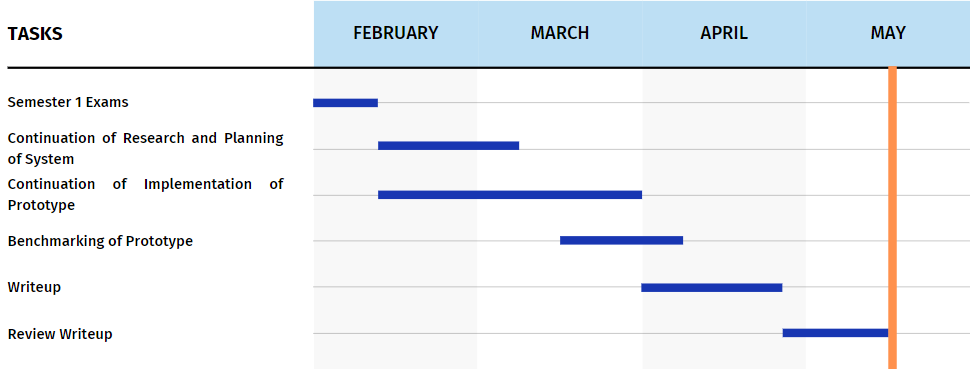
\includegraphics[width=\textwidth]{gantt.png}
\caption{Gantt Chart for Second Semester}
\centering
\end{figure}
Several experiments will be carried out to empirically measure the response times of the actors under varying computational load to assess the system’s scalability. The time and space complexity and generated network traffic will also be analysed to measure the footprint the framework has on the devices it is running on. Moreover, a case study will be done to perform a qualitative comparison between JavaScript code using the actor model to plain JavaScript. The experiments will add to the existing evidence of the practicality of implementing the actor model framework in JavaScript. The experiments will also assess the system's performance and scalability through quantitative analysis. Finally, through the qualitative case study the usability of the actor model will be shown when using JavaScript on the web.
\section{Deliverables}
The deliverables of this project will be included in a GitHub repository containing the implementation of the project (see \url{https://github.com/Android2771/fyp}). The repository will also include applications or configurations to benchmark the system as well as the \LaTeX~file for the Final Year Project documentation. The Final Year Report will be provided separately as per the provided schedule requirements.
\bibliographystyle{ieeetr}
\bibliography{references}  
\end{document}